\begin{table*}[t]
\small
\setlength{\tabcolsep}{3pt}
\centering
\begin{tabular}{l | r r r r | r r r r}
\toprule
 & \multicolumn{4}{c|}{\textbf{7B-4T}} & \multicolumn{4}{c}{\textbf{13B-5T}} \\
& \multicolumn{2}{c}{BPB} & \multicolumn{2}{c|}{TaskCE} & \multicolumn{2}{c}{BPB} & \multicolumn{2}{c}{TaskCE} \\
& Error &  \%Error & Error &  \%Error & Error &  \%Error & Error &  \%Error  \\
\midrule
MMLU & 0.6 & 1.3\% & 9.0 & 18.3\% & 0.3 & 0.6\% & 10.4 & 20.2\% \\
HellaSwag & 1.2 & 1.4\% & 5.9 & 7.2\% & 2.1 & 2.5\% & 8.7 & 10.5\% \\
ARC-Challenge & 10.4 & 16.9\% & 13.1 & 21.3\% & 11.1 & 17.5\% & 12.3 & 19.5\% \\
ARC-Easy & 8.0 & 9.4\% & 4.5 & 5.4\% & 10.0 & 11.4\% & 5.4 & 6.2\% \\
PIQA & 0.8 & 1.0\% & 2.5 & 3.1\% & 0.9 & 1.1\% & 2.4 & 2.9\% \\
CommonsenseQA & 3.1 & 4.2\% & 1.9 & 2.6\% & 3.5 & 4.7\% & 2.0 & 2.7\% \\
Social IQa & 1.2 & 2.0\% & 0.5 & 0.7\% & 1.7 & 2.7\% & 0.8 & 1.2\% \\
OpenBookQA & 5.2 & 10.6\% & 3.5 & 7.1\% & 3.7 & 7.8\% & 0.1 & 0.2\% \\
\bottomrule
\end{tabular}
\caption{
    Comparison of original and new prediction errors for 7B-4T and 13B-5T models across tasks. Absolute (Error) and relative (\%Error) differences are shown.
}
\label{tab:updated_pred_taskce}
\end{table*}


\begin{figure*}[ht]
    \centering
    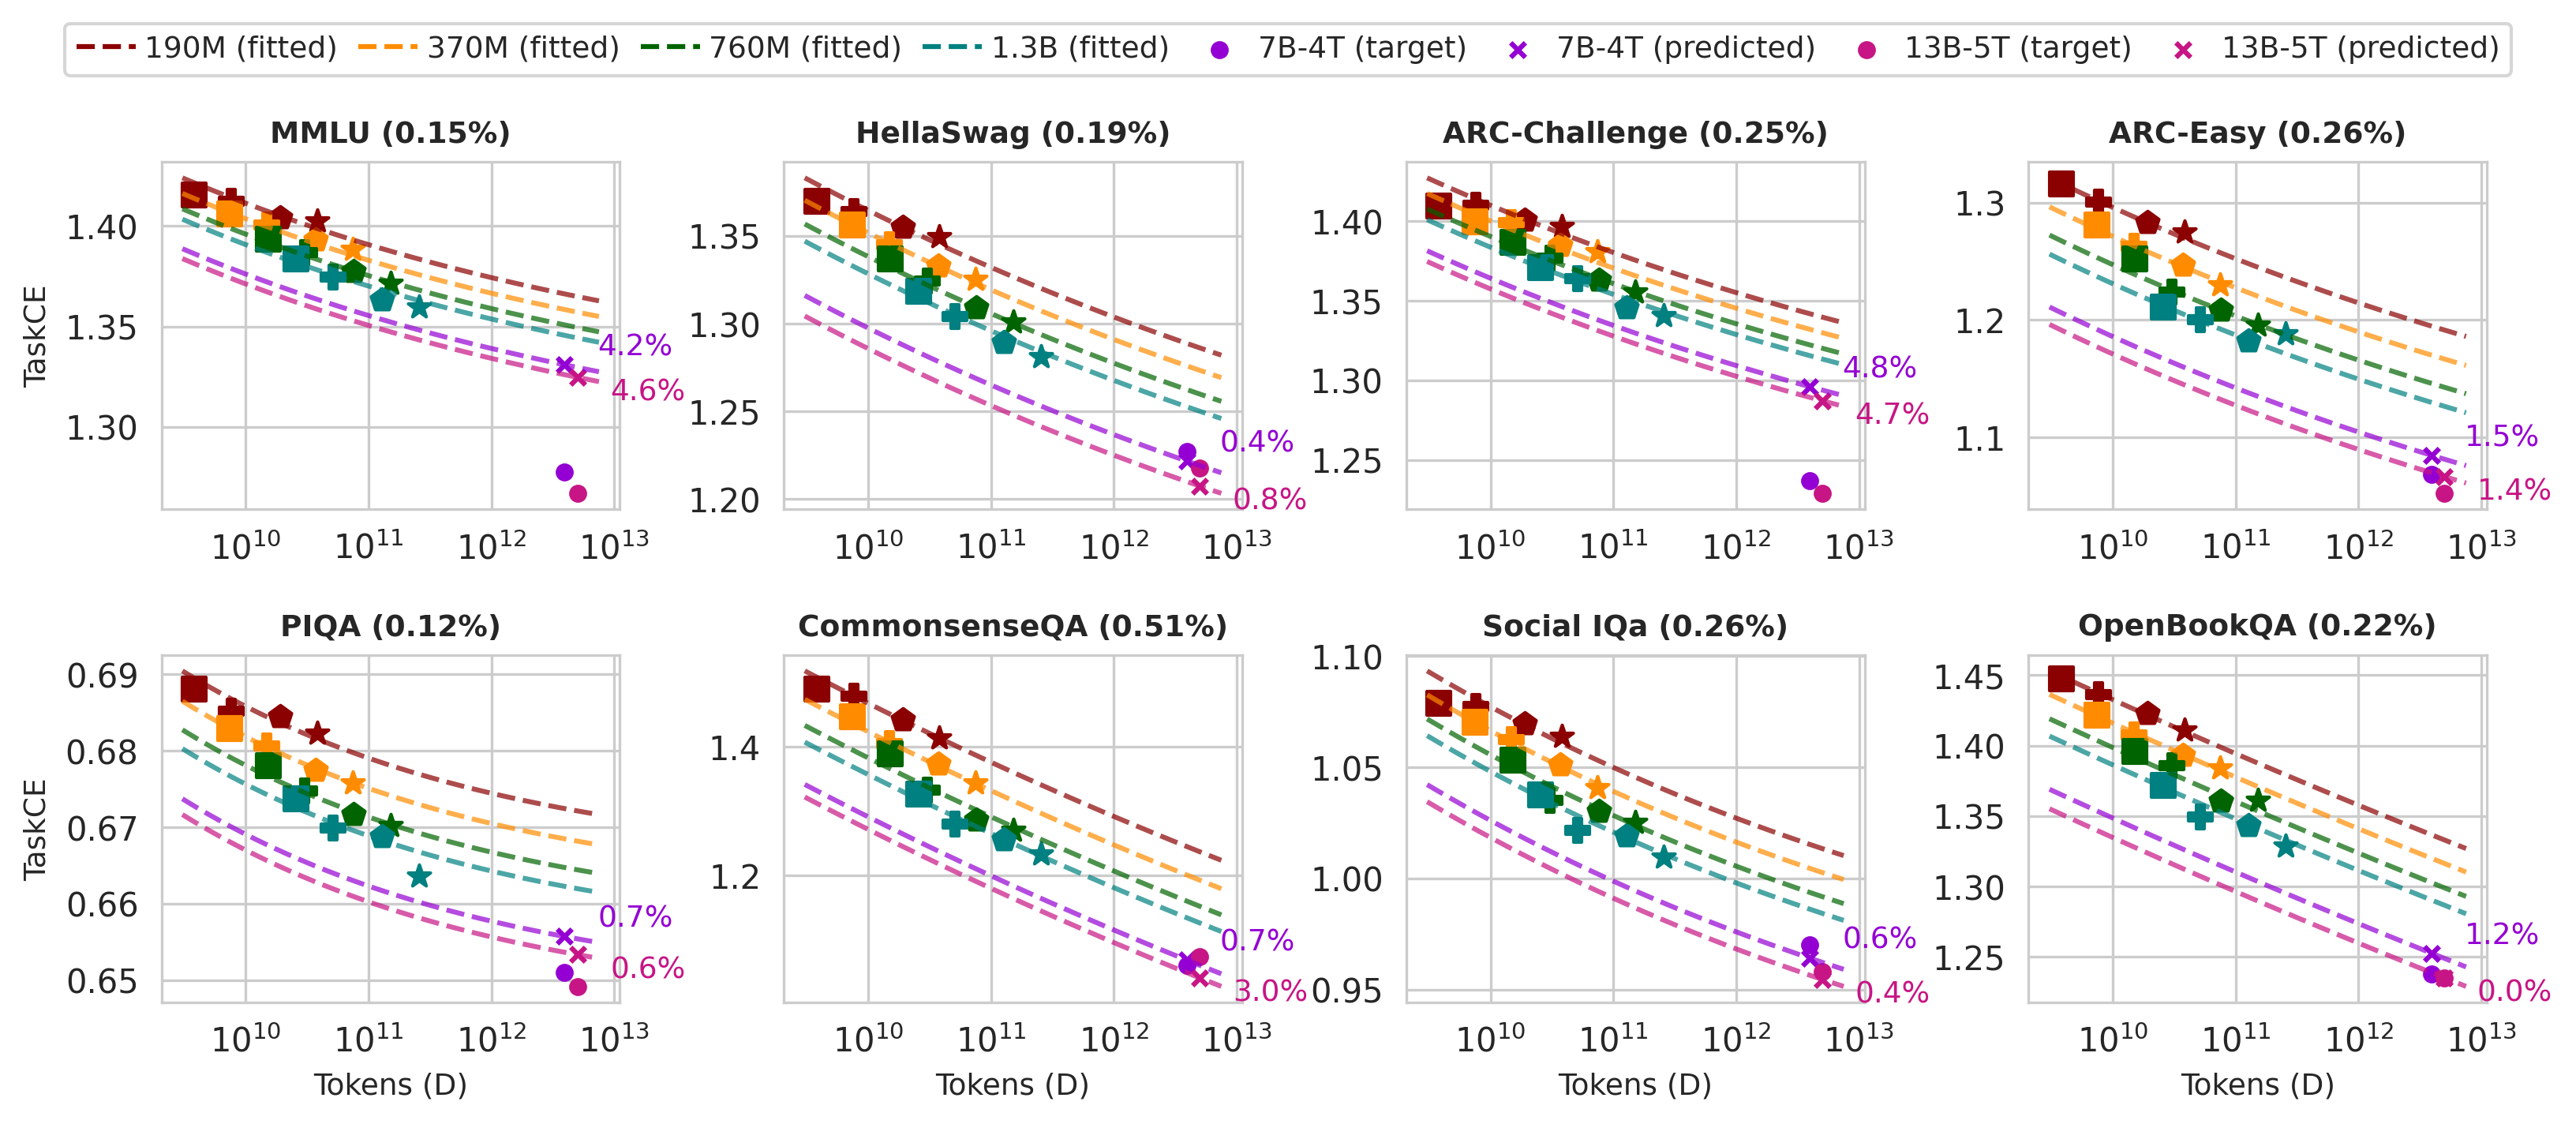
\includegraphics[width=\linewidth]{images/step1_taskce_main.png}
    \caption{Predicting final \textit{task cross-entropy} (\autoref{eqn:task_ce}) from model parameters and token budget in step 1.}
    \label{fig:step1_taskce}
\end{figure*}


\begin{figure*}[ht]
    \centering
    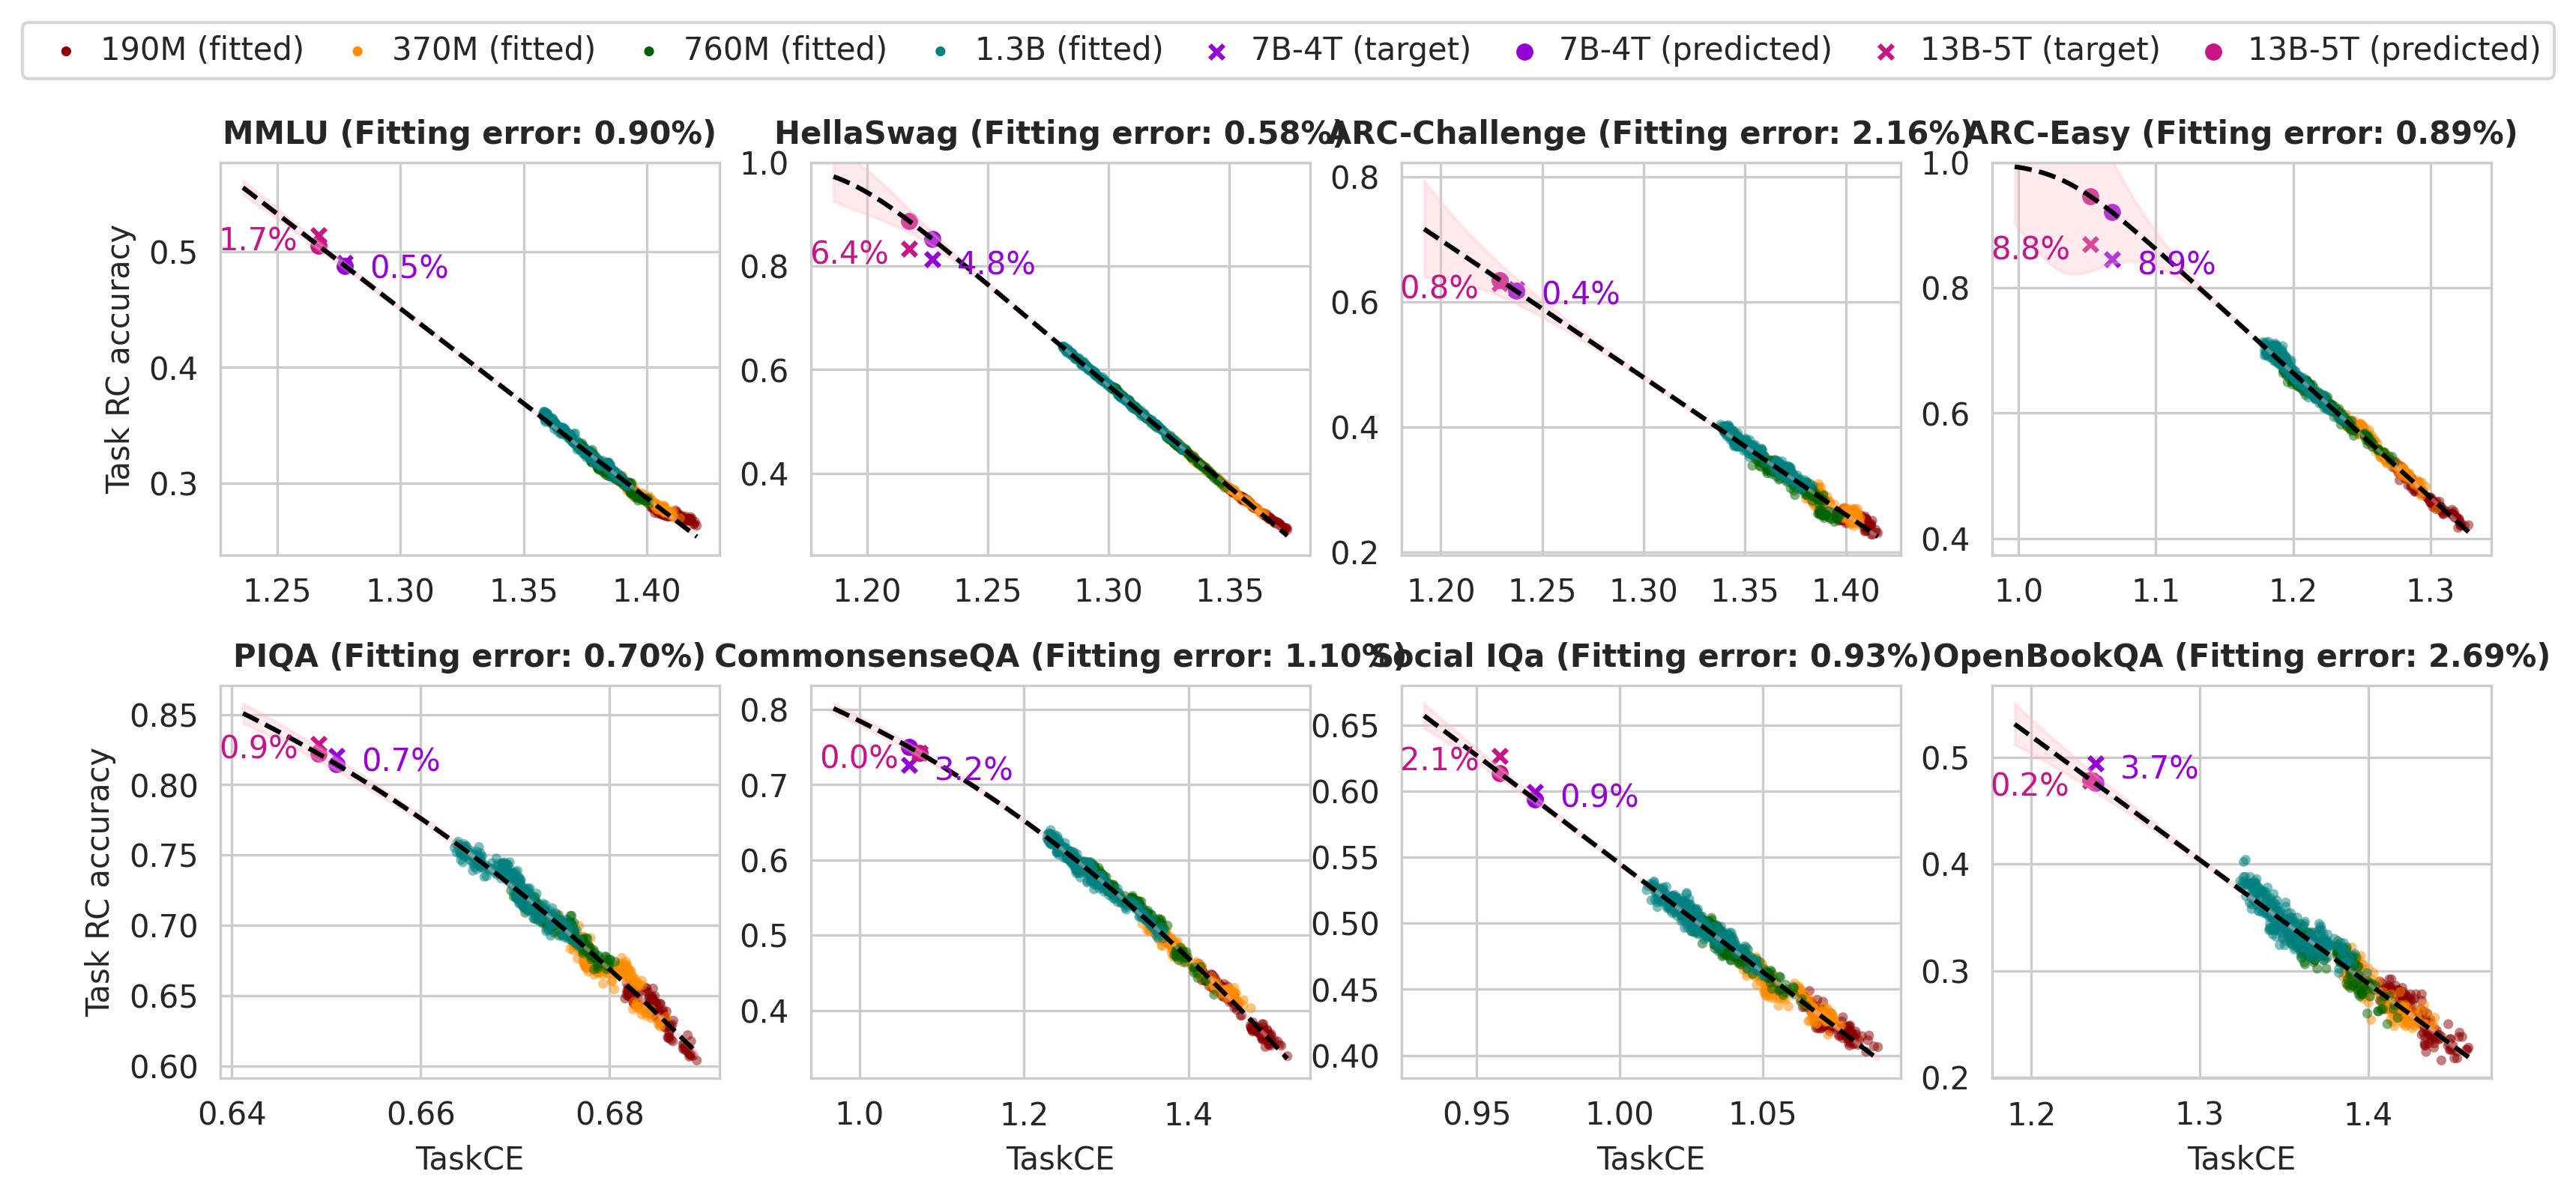
\includegraphics[width=\linewidth]{images/step2_taskce_main.png}
    \caption{Predicting the task metric from the \textit{task cross-entropy} (\autoref{eqn:task_ce}) in step 2.}
    \label{fig:step2_taskce}
\end{figure*}


\begin{figure*}[ht]
    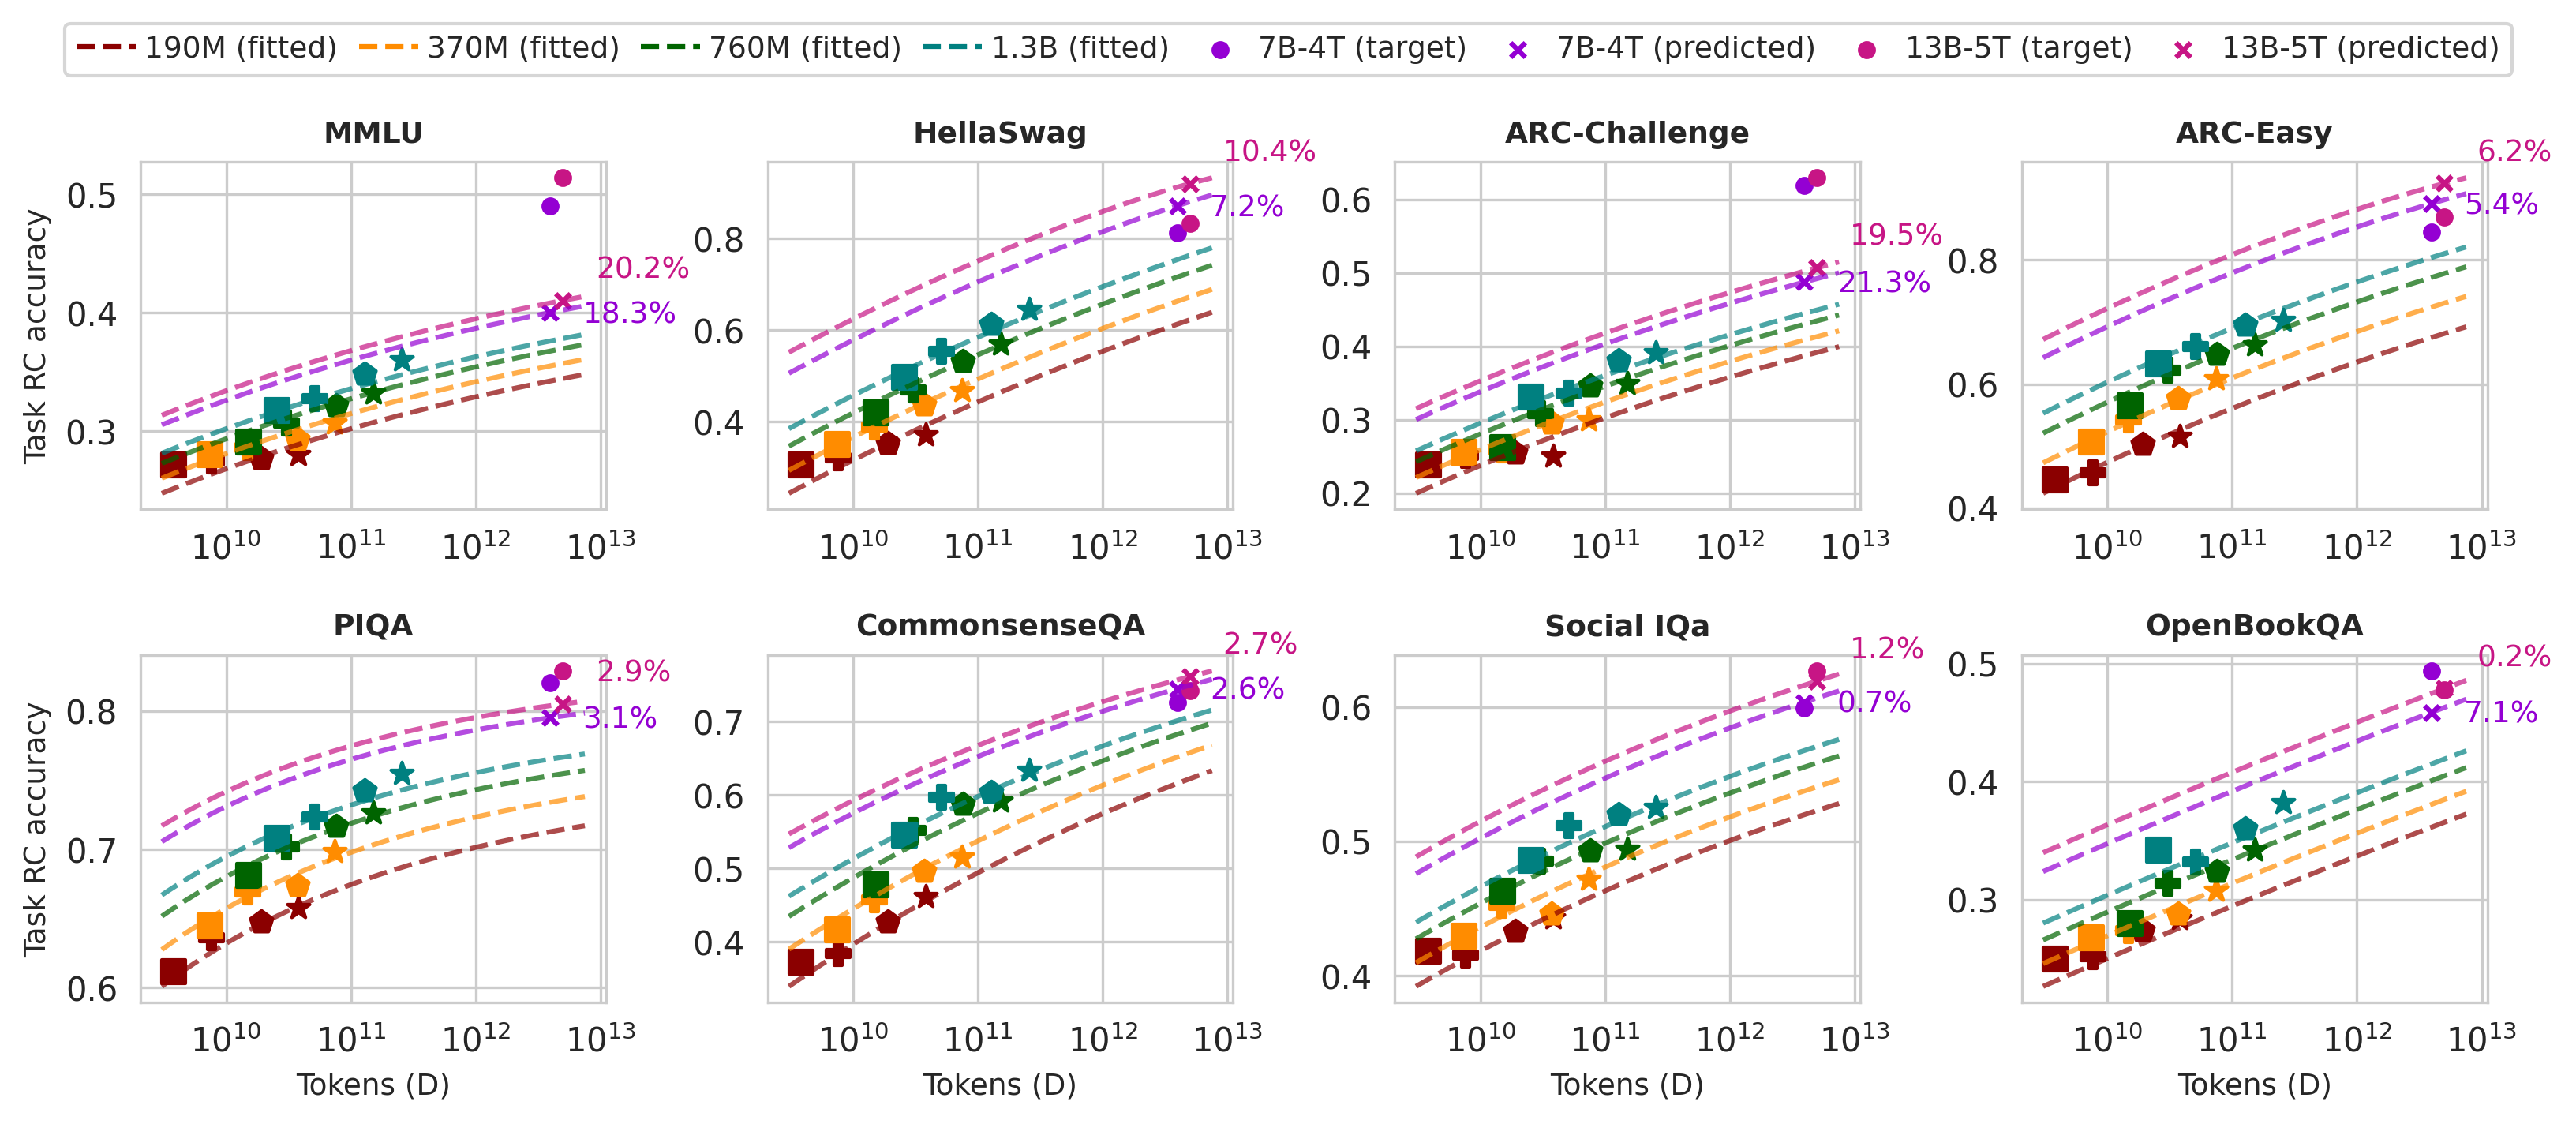
\includegraphics[width=\linewidth]{images/chained_taskce_main.png}
    \caption{Chaining predictions from step 1 (\autoref{fig:step1_taskce}) and step 2 (\autoref{fig:step2_taskce}) with \textit{task cross-entropy} as the intermediate feature.}
    \label{fig:chained_taskce}
\end{figure*}